\documentclass[11pt]{article}

\usepackage[margin=1in]{geometry}
\usepackage{enumitem}
\usepackage{hyperref}
\usepackage{microtype}
\usepackage{tikz}
\usetikzlibrary{arrows.meta}

\setlist[itemize]{nosep,leftmargin=*}
\setlist[enumerate]{nosep,leftmargin=*}

% ---- Fill these in before submitting ----
\newcommand{\StudentName}{Muhammad\ Abdullah}
\newcommand{\StudentID}{BSCS23070}

\title{Building Resilient Distributed Systems: StudySync}
\author{\StudentName\ (\StudentID)}
\date{May 5, 2026}

\begin{document}
\maketitle

\section*{Part 1 --- Analyze the Mess (Root Causes)}

\subsection*{Problem 1: Synchronization (Lost Update)}
\begin{itemize}
  \item \textbf{Root cause:} the backend performs a read--modify--write cycle without any concurrency control.
  Two clients can read the same document state and then both write; the later write overwrites the earlier one.
  \item \textbf{Where it happens:} at the database write boundary (e.g., \texttt{UPDATE documents SET ... WHERE id=?})
  without a version predicate and without detecting write conflicts.
  \item \textbf{Failure mode:} \emph{last-write-wins} silently violates user expectations; the API returns 200 even though it
  discarded one user's edits.
\end{itemize}

\subsection*{Problem 2: Coordination (Dropped Clerk Webhook)}
\begin{itemize}
  \item \textbf{Root cause:} the system treats a webhook as a reliable one-shot message.
  If the cancellation event is dropped (or the handler crashes mid-processing), the backend never learns the state transition.
  \item \textbf{Why it becomes permanent:} there is no durable event log (``inbox''), no idempotency key storage, and no retry/DLQ.
  Therefore the missing transition is never replayed, so the database remains stale forever.
\end{itemize}

\subsection*{Problem 3: Fault Tolerance (LLM Timeout Hangs the App)}
\begin{itemize}
  \item \textbf{Root cause:} synchronous outbound calls to the LLM with long timeouts block request workers.
  \item \textbf{Distributed consequence:} when the LLM slows or fails, requests pile up, latency spikes, and the server becomes effectively unavailable
  due to thread/worker exhaustion.
\end{itemize}

\section*{Part 2 --- Design a Better System}

\subsection*{Fix for Problem 1: Optimistic Locking (Versioned Writes)}
\begin{itemize}
  \item Add an integer \texttt{version} column to each shared document row.
  \item API contract: every \texttt{PUT/PATCH} includes \texttt{expectedVersion}.
  \item Database update becomes conditional:
  \begin{center}
    \texttt{UPDATE documents SET content=?, version=version+1 WHERE id=? AND version=?}
  \end{center}
  \item If 0 rows are updated, return \texttt{409 Conflict} with the latest version so the client can re-fetch and retry.
\end{itemize}

\subsubsection*{UML Sequence Diagram (Two Concurrent Editors)}
\begin{center}
\footnotesize
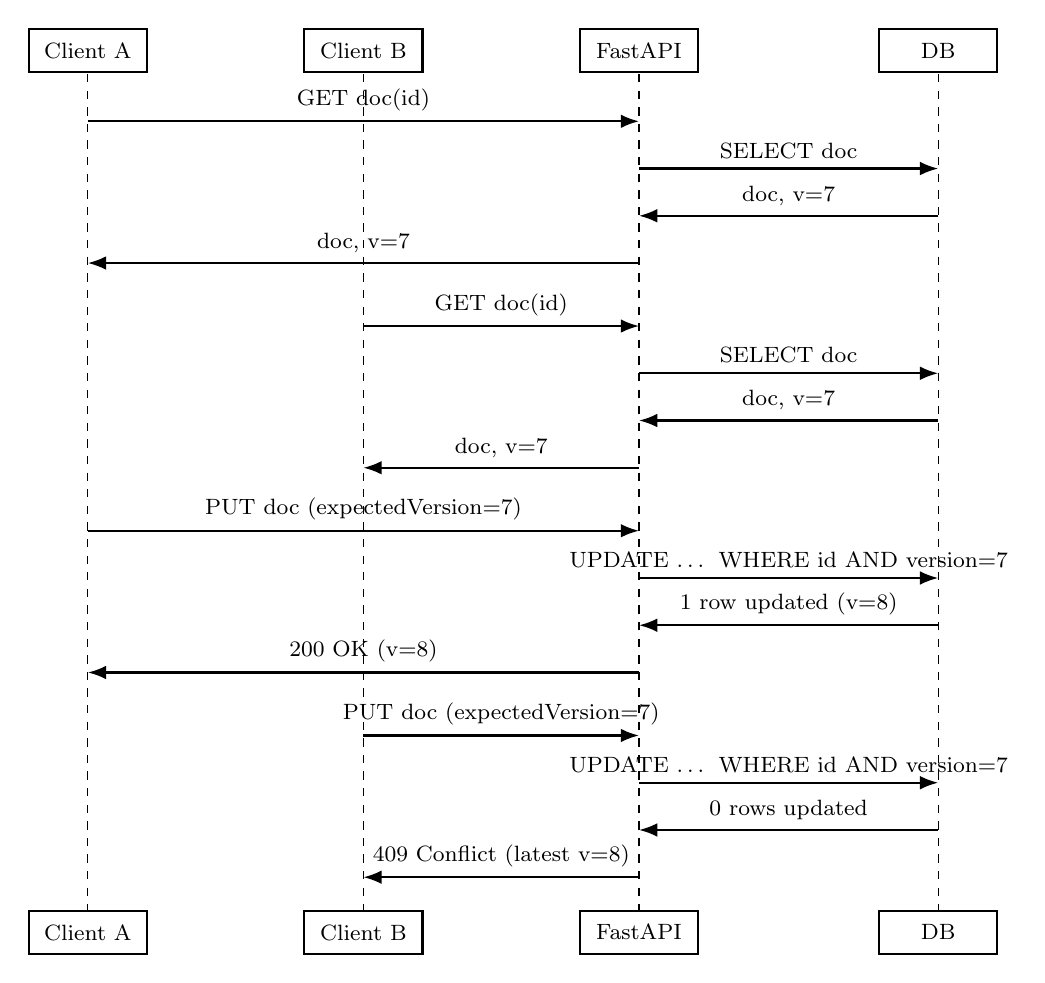
\begin{tikzpicture}[
  >=Latex,
  every node/.style={font=\footnotesize},
  participant/.style={rectangle, draw, thick, minimum width=1.5cm,
                      minimum height=0.55cm, align=center, fill=white},
  msg/.style={->, thick}
]

\def\seqXA{0}
\def\seqXB{3.5}
\def\seqXAPI{7}
\def\seqXDB{10.8}

\node[participant] at (\seqXA, 0)   (boxA)   {Client A};
\node[participant] at (\seqXB, 0)   (boxB)   {Client B};
\node[participant] at (\seqXAPI, 0) (boxAPI) {FastAPI};
\node[participant] at (\seqXDB, 0)  (boxDB)  {DB};

\draw[dashed, thin] (\seqXA,  -0.3) -- (\seqXA,  -11.2);
\draw[dashed, thin] (\seqXB,  -0.3) -- (\seqXB,  -11.2);
\draw[dashed, thin] (\seqXAPI,-0.3) -- (\seqXAPI,-11.2);
\draw[dashed, thin] (\seqXDB, -0.3) -- (\seqXDB, -11.2);

\draw[msg] (\seqXA, -0.9)  -- (\seqXAPI,-0.9)  node[midway,above]{GET doc(id)};
\draw[msg] (\seqXAPI,-1.5) -- (\seqXDB, -1.5)  node[midway,above]{SELECT doc};
\draw[msg] (\seqXDB, -2.1) -- (\seqXAPI,-2.1)  node[midway,above]{doc, v=7};
\draw[msg] (\seqXAPI,-2.7) -- (\seqXA,  -2.7)  node[midway,above]{doc, v=7};

\draw[msg] (\seqXB,  -3.5) -- (\seqXAPI,-3.5)  node[midway,above]{GET doc(id)};
\draw[msg] (\seqXAPI,-4.1) -- (\seqXDB, -4.1)  node[midway,above]{SELECT doc};
\draw[msg] (\seqXDB, -4.7) -- (\seqXAPI,-4.7)  node[midway,above]{doc, v=7};
\draw[msg] (\seqXAPI,-5.3) -- (\seqXB,  -5.3)  node[midway,above]{doc, v=7};

\draw[msg] (\seqXA,  -6.1) -- (\seqXAPI,-6.1)
           node[midway,above]{PUT doc (expectedVersion=7)};
\draw[msg] (\seqXAPI,-6.7) -- (\seqXDB, -6.7)
           node[midway,above]{UPDATE \ldots{} WHERE id AND version=7};
\draw[msg] (\seqXDB, -7.3) -- (\seqXAPI,-7.3)
           node[midway,above]{1 row updated (v=8)};
\draw[msg] (\seqXAPI,-7.9) -- (\seqXA,  -7.9)  node[midway,above]{200 OK (v=8)};

\draw[msg] (\seqXB,  -8.7) -- (\seqXAPI,-8.7)
           node[midway,above]{PUT doc (expectedVersion=7)};
\draw[msg] (\seqXAPI,-9.3) -- (\seqXDB, -9.3)
           node[midway,above]{UPDATE \ldots{} WHERE id AND version=7};
\draw[msg] (\seqXDB, -9.9) -- (\seqXAPI,-9.9)  node[midway,above]{0 rows updated};
\draw[msg] (\seqXAPI,-10.5)-- (\seqXB,  -10.5)
           node[midway,above]{409 Conflict (latest v=8)};

\node[participant] at (\seqXA,  -11.2) {Client A};
\node[participant] at (\seqXB,  -11.2) {Client B};
\node[participant] at (\seqXAPI,-11.2) {FastAPI};
\node[participant] at (\seqXDB, -11.2) {DB};

\end{tikzpicture}
\end{center}

\subsection*{Fix for Problem 2: Fault-Tolerant Webhook Handling (Inbox + Idempotency + Retry/DLQ)}
\begin{itemize}
  \item \textbf{Inbox table:} persist every verified webhook event in a \texttt{webhook\_events} table with a \textbf{unique} \texttt{event\_id}
  (e.g., Svix/Clerk's delivery id). This makes delivery \emph{durable}.
  \item \textbf{Idempotency:} if an event id is seen again, do not re-insert; safely re-process only if needed.
  \item \textbf{Retry with backoff:} store \texttt{attempts} and \texttt{next\_attempt\_at}; retry transient failures.
  \item \textbf{Dead-letter queue (DLQ):} after $N$ failed attempts, mark the event \texttt{dead} for manual inspection.
  \item \textbf{Optional reconciliation:} periodically query Clerk for authoritative subscription state to heal rare cases where
  a webhook was never delivered.
\end{itemize}

\subsection*{Fix for Problem 3: Circuit Breaker + Fallback for LLM Calls}
\begin{itemize}
  \item Wrap outbound LLM calls with: (1) short timeouts, (2) a circuit breaker (open after repeated failures),
  and (3) a fallback response.
  \item When the circuit is open, return a fast fallback (e.g., cached example challenge, or a ``try again later'' message)
  so the rest of the API remains responsive.
\end{itemize}

\subsection*{CAP Trade-offs (Quick Discussion)}
\begin{itemize}
  \item \textbf{Optimistic locking:} prefers \textbf{Consistency} for shared edits (conflicts return 409) at the cost of some \textbf{Availability}
  during contention (clients must retry).
  \item \textbf{Webhook inbox + retries:} prefers \textbf{Availability} of the webhook endpoint (ack quickly after persisting)
  while achieving \textbf{eventual consistency} between Clerk and the local DB.
  \item \textbf{Circuit breaker:} prefers \textbf{Availability/Latency} over strict completeness when the LLM is unhealthy.
\end{itemize}

\section*{Part 3 --- Code Implemented}
I implemented \textbf{Problem 2 (Coordination)} in the FastAPI backend using an inbox table (durable event storage),
idempotency, and a retryable processor so a transient failure cannot permanently desynchronize Clerk and the local database.

\subsection*{Implementation Summary (Backend)}
\begin{itemize}
  \item \textbf{Webhook endpoint acknowledges quickly:} \texttt{POST /webhooks/clerk} verifies the Svix/Clerk signature,
  then persists the event and immediately returns \texttt{accepted}. Processing is not done inline, so a slow DB or transient
  exception does not cause Clerk to time out and drop the event.

  \item \textbf{Durable inbox table:} every delivery is stored in \texttt{webhook\_events} with a \textbf{unique} \texttt{event\_id}
  (preferring the Svix header id). This is the idempotency key: if Clerk retries the same delivery, insertion becomes a no-op.

  \item \textbf{Retry with backoff + DLQ:} the processor reads events with \texttt{status=pending} and
  \texttt{next\_attempt\_at} $\leq$ \texttt{now}.
  If processing fails, it increments \texttt{attempts}, records \texttt{last\_error}, and schedules the next attempt using exponential backoff.
  After $N$ attempts, the event is marked \texttt{dead} (dead-letter) for manual inspection.

  \item \textbf{Local state update:} for subscription cancellation events, the handler updates a local entitlement row
  (\texttt{user\_entitlements.is\_premium=false}). This turns an unreliable, one-shot webhook into a reliable state transition.
\end{itemize}

\subsection*{Failure Simulation (Proof)}
\begin{itemize}
  \item A unit test inserts a cancellation event into the inbox and intentionally forces the first processing attempt to fail
  (simulated transient error). The event remains \texttt{pending} with \texttt{attempts=1}.
  \item On the next processing pass, the event succeeds and the entitlement becomes non-premium, demonstrating that a transient failure
  does not cause permanent inconsistency.
\end{itemize}

\end{document}
